\documentclass[handout]{beamer} % use [handout] option to stop pauses
\beamertemplatenavigationsymbolsempty 

\usepackage[utf8]{inputenc}
\usepackage{svg}
\usepackage{amsmath}
\usepackage{amssymb}
\usepackage{mathtools}
\usepackage{stmaryrd}
\usepackage{libertine}
\usepackage{xparse}
\usepackage{mathpartir}
\usepackage{fancybox}
\usepackage{graphicx}
\usepackage{tikz}
\usepackage{../jmsdelim}
\usepackage{../macros}
\usepackage{../categories}

\usecolortheme[named=BristolURed]{structure}

\AtBeginSection[]{
  \begin{frame}
  \vfill
  \centering
  \begin{beamercolorbox}[sep=12pt,center,shadow=true]{title}
		\usebeamerfont{title}
		\scshape
		\uppercase\expandafter{\romannumeral\insertsectionnumber\relax}.~\insertsectionhead\par%
  \end{beamercolorbox}
  \vfill
  \end{frame}
}

\newcommand\doubleplus{+\kern-1.3ex+\kern0.8ex}

\title{Type Theory and Homotopy \\ III. Equivalences, Univalence, and Quotients}
\author{
		Alex Kavvos % \inst{1} % \orcidID{0000-0001-7953-7975}
}

% \institute{
% 		% \inst{1}
%     University of Bristol
% 		% \email{alex.kavvos@bristol.ac.uk}
% }
\titlegraphic{
\includegraphics[scale=0.1]{../Bristol.png}}
\date{Panhellenic Logic Symposium, 6--10 July 2022}


\begin{document}

\frame{\titlepage}

\begin{frame}
  \frametitle{Previously}

  Intensional identity types seem to support the following view:
  \begin{itemize}
    \item Types are \textbf{spaces} (up to homotopy).
    \item Terms are \textbf{points}.
    \item Elements of the identity type are \textbf{paths}.
    \item Everything given in a \textbf{synthetic} manner, not analytic.
  \end{itemize}
  
  This discovery is independently due to 
  \begin{itemize}
    \item Awodey and Warren [Math. Proc. Camb. Philos. Soc. 2009]
    \item Vladimir Voevodsky (1966--2017) [Stanford lecture 2006]
  \end{itemize}
  
  Interpretation of TT into \textbf{simplicial sets}: Kapulkin and Lumsdaine,
  with thanks to Voevodsky [J. Eur. Math. Soc. 2018].
  
  \medskip
  
  % But Voevodsky discovered that simplicial sets support a little bit more than MLTT\ldots
\end{frame}




\section{Homotopical structure of types}

\begin{frame}
  \frametitle{Homotopy Levels}

  Types are spaces; they have \textbf{higher-dimensional structure}.
  
  \medskip
  
  Yet, some types do not. Let $A$ be a type.
  \begin{align*}
    \alert{contractible} && \Sfn{isContr}{A} &\defeq
      \DSum{c}{A}{
        \parens{
          \Fn{x}{A}{
            \Id{A}{c}{x}
          }
        }
      }
    \\
    \text{proposition} && \Sfn{isProp}{A} &\defeq
      \Fn{x, y}{A}{
        \Id{A}{x}{y}
      }
    \\
    \text{set} && \Sfn{isSet}{A} &\defeq
      \Fn{x, y}{A}{
        \Fn{p, q}{\Id{A}{x}{y}}{
          \Id{}{p}{q}
        }
      }
    \\
    && \vdots & 
  \end{align*}
  In general, we define
  \begin{align*}
    \Sfn{is-(-2)-type}{A} &\defeq \Sfn{isContr}{A} \\
    \Sfn{is-(n+1)-type}{A} &\defeq \Fn{x, y}{A}{\Sfn{isContr}{\Id{A}{x}{y}}}
  \end{align*}
  Then 
  \begin{align*}
    \Sfn{is-(-1)-type}{A} &\simeq \Sfn{isProp}{A}
    &
    \Sfn{is-0-type}{A} &\simeq \Sfn{isSet}{A}
  \end{align*}
\end{frame}

\begin{frame}
  \frametitle{Propositions and Sets}

  Here is an unusual result:

  \begin{theorem}[Hedberg, J. Func. Prog 1998]
    Let $A$ be a type. If \textbf{identity is decidable}, i.e. if we have
    \[
      d : \Fn{x, y}{A}{\Id{A}{x}{y} + \lnot\Id{A}{x}{y}}
    \]
    then $A$ \textbf{is a set}, i.e. we have a proof of $\Sfn{isSet}{A}$.
  \end{theorem}

  \begin{corollary}
    $\Nat$ is a set.
  \end{corollary}
  
  \medskip
  In some sense, all the maths we have done so far is \textbf{0-dimensional}!
\end{frame}


\section{Universes}


\begin{frame}
  \frametitle{Identity types are not good enough}
  
  \begin{theorem}[Jan Smith, J. Symb. Log. 1988]
    The type correspondong to Peano's fourth axiom, i.e.
    \[
      \IsTy[n : \Nat]{\Id{\Nat}{0}{\Succ{n}} \to \mathbf{0}}[]
    \]
    is \textbf{not} inhabited in MLTT with $\to$, $\times$, and identity types.
  \end{theorem}
  Proof: construct a model of MLTT where types are subsingleton sets.

  \medskip

  To prove Peano 4, we intuitively want to
  \begin{enumerate}
    \item \Alert{construct a type family} $\IsTy[n : \Nat]{B(n)}[]$ where
      \begin{align*}
        \IsTy[]{\,&B(\Tm{\Zero})}[] && \quad\text{ is inhabited} \\
        \IsTy[n : \Nat]{\,&B(\Tm{\Succ{n}})}[] && \quad\text{ is  empty, i.e.} \deq \mathbf{0}
      \end{align*}
    \item assuming $\IsTm[n : \Nat]{P}{\Id{\Nat}{0}{\Succ{n}}}$ and
      $\IsTm[]{M}{B(\Tm{\Zero})}$, obtain $\IsTm[n :
      \Nat]{\App{\Transport{P}}{M}}{B(\Tm{\Succ{n}})} \deq \textbf{0}$
  \end{enumerate}
  We cannot perform Step 1 because types are not terms.
\end{frame}

\begin{frame}
  \frametitle{Universes \`{a} la Russell}
  We introduce the \textbf{universe}, a \textbf{type of all (small) types}.
  \begin{mathpar}
    \inferrule{ }{\IsTy{\Uni}[]}
    \and
    \inferrule{
      \IsTm{A}{\Uni}
    }{
      \IsTy{A}[]
    }
  \end{mathpar}
  plus one rule for each type constructor, e.g.
  \begin{mathpar}
    \inferrule{
      \IsTm{A}{\Uni} \\
      \IsTm[\Gamma, x : \Uni]{B}{\Uni}
    }{
      \IsTm{\Fn{x}{A}{B}}{\Uni}
    }
  \end{mathpar}
  \Alert{Caution}. We must \textbf{avoid} the following to avoid paradoxes:
  \[
    \inferrule{ }{\IsTm{\Uni}{\Uni}}
  \]
  
  Types may then be constructed as terms of $\Uni$ (e.g. by induction).
  
  \medskip
  
  If $A : \Uni$ then we say that $A$ is a \textbf{small} type.
\end{frame}

\begin{frame}
  \frametitle{Homotopy equivalence}

  \begin{definition}
    Two topological spaces $X$ and $Y$ are \textbf{homotopy-equivalent} if there
    are continuous functions $f : X \to Y$ and $g : Y \to X$ such that
    \begin{align*}
      g \circ f &\sim 1_X 
      &
      f \circ g &\sim 1_Y
    \end{align*}
    where $1_X$ and $1_Y$ are the identity functions on $X$ and $Y$.
  \end{definition}

  \begin{center}
    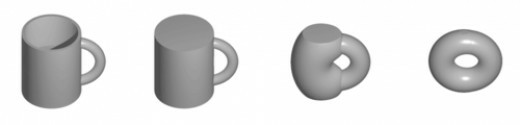
\includegraphics[scale=0.3]{mug.jpg}
  \end{center}
  
  We can model this synthetically in MLTT.
\end{frame}

\begin{frame}
  \frametitle{Type-theoretic Equivalences}

  \begin{definition}[Voevodsky]
    We say that $f : A \to B$ is an \textbf{equivalence} just if
    \[
      \IsEquiv{f} \defeq
        \Fn{y}{B}{
          \Sfn{isContr}{
            \DSum{x}{A}{\Id{B}{f(x)}{y}}
          }
        }
    \]
  \end{definition}

  This is a homotopically well-behaved notion of \textbf{isomorphism}.
  
  \medskip
  
  For $A, B : \Uni$ define the type of \textbf{(type-theoretic) equivalences}
  \[
    A \simeq B \defeq
      \DSum{f}{A \to B}{\IsEquiv{f}}
  \]
  
  We can use equivalences to \textbf{decompose} identity types.
  
  \medskip

  E.g. for any $A, B : \Uni$ and $p, q : A \times B$:
  \begin{align*}
    \Id{A \times B}{p}{q} &\simeq 
    \Id{A}{\Proj[1]{p}}{\Proj[1]{q}} \times \Id{B}{\Proj[2]{p}}{\Proj[2]{q}}
  \end{align*}
  
  This can be done for most type formers of MLTT.
  
\end{frame}

\begin{frame}
  \frametitle{Univalence}
  
  Question:
  \begin{center}
    \shadowbox{What is an identity between types?}
  \end{center}
  
  Voevodsky proposed adding the \textbf{univalence axiom} to MLTT:
  \[
    \textsf{ua} : 
      \Fn{A, B}{\Uni}{
        (A \simeq B) \simeq \Id{\Uni}{A}{B}
      }
  \]
  This spoils the computational character of MLTT, but is a revolution:
  
  \begin{center}
    \shadowbox{isomorphic/equivalent types are identical}
  \end{center}
  This principle is often used informally in maths (`abuse of notation').

  E.g. the Cauchy reals and the Dedekind reals are ``the same.''
  
  \medskip

  Its soundness is validated by the simplicial model of type theory.
  (The identity type elimination rule remains valid!)
\end{frame}

% \begin{frame}
%   \frametitle{Type-theoretic homotopies}

%   Let $A, B : \Uni$ and $f, g : A \to B$. 
  
%   \medskip
  
%   Define the type of \textbf{(type-theoretic) homotopies} from $f$ to $g$ to be
%   \[
%     f \sim g \defeq
%       \Fn{x}{A}{
%         \Id{B}{\App{f}{x}}{\App{g}{x}}
%       }
%   \]
% \end{frame}

\section{Quotients}

\begin{frame}
  \frametitle{Quotients}

  It is in general difficult to form \textbf{quotients} in MLTT.
  
  \medskip
  
  Quotient types:
  \begin{mathpar}
    \small
    \inferrule{
      \IsTy{A}[]\\
      \IsTy[\Gamma, x : A, y : A]{R}[]
    }{
      \IsTy{A/R}[]
    }
    \and
    \inferrule{
      \IsTm{M}{A} \\
      \IsTy{A/R}
    }{
      \IsTm{[M]}{A/R}
    }
    \and
    \inferrule{
      \IsTm{M, N}{A} \\
      \IsTy[\Gamma, x : A, y : A]{R}[] \\
      \IsTm{P}{\Sb{R}{M, N}{x, y}}
    }{
      \IsTm{\textsf{Qax}(P)}{\Id{A/R}{[M]}{[N]}}
    }
  \end{mathpar}
  and so on... but such types are not necessarily \textbf{effective}:
  \begin{mathpar}
    \small
    \inferrule{
      \IsTy[\Gamma, x : A, y : A]{R(x, y)}[] \\
      \IsTm{P}{\Id{A/R}{[M]}{[N]}}
    }{
      \IsTm{\textsf{???}(M, N, P)}{R(\Tm{M}, \Tm{N})}
    }
  \end{mathpar}
  Worse:
  \begin{theorem}[Maietti 1999]
    If quotient types are effective and UIP holds then $A + \lnot A$ for small $A$.
  \end{theorem}
  
\end{frame}

\begin{frame}
  \frametitle{Higher Inductive Types (HITs)}

  Idea:
  \begin{center}
    \shadowbox{When building a type, also specify some paths.}
  \end{center}
  
  For example, to build a type $\Int$ of integers we may postulate:
  \begin{itemize}
    \item for each $\Tm{M} : \Nat$ a \textbf{positive integer} $\Tm{\Sfn{pos}{M}} : \Int$
    \item for each $\Tm{M} : \Nat$ a \textbf{negative integer} $\Tm{\Sfn{neg}{M}} : \Int$
    \item an identity $\Tm{\textsf{pnZero}} : \Id{\Int}{\Sfn{pos}{\Zero}}{\Sfn{int}{\Zero}}$  
  \end{itemize}
  
  \medskip
  
  This can be used to specify homotopical spaces synthetically.

  E.g. a circle can be specified by postulating
  \begin{itemize}
    \item a base point $\Tm{\textsf{base}} : \mathbb{S}^1$
    \item a path $\Tm{\textsf{loop}} : \Id{\mathbb{S}^1}{\textsf{base}}{\textsf{base}}$
  \end{itemize}
  This leads to \textbf{synthetic homotopy theory}.
  E.g. there is a machine-checked proof that $\pi_4(\mathbb{S}^3) \simeq \mathbb{Z}_2$.
\end{frame}

\begin{frame}
  \frametitle{Homotopy Type Theory (HoTT)}
  
  The results of Awodey/Warren/Voevodsky led to a flurry of results.

  This culminated in a Special Year at the IAS in Princeton:
  
  \begin{center}
    
\includegraphics[scale=0.7]{hott.png}
  \end{center}
  
  \[
    \text{HoTT} \defeq \text{MLTT} + \text{univalence axiom} + \text{some HITs}
  \]

\end{frame}


\section{Further directions}

\begin{frame}
  \frametitle{50 Years of MLTT}
  
  Achievements:
  \begin{itemize}
    \item A number of well-behaved type theories\ldots
    \item \ldots with well-understood semantics.
    \item One industrial-strength proof assistant: \textbf{Coq}.
      
    Many machine-checked proofs! Greatest hits:
    \begin{itemize}
      \item Four color theorem [Gonthier 2008]
      \item Feit-Thompson odd order theorem [Gonthier et al. 2013]
      \item CompCert, a verified C compiler [Leroy et al. 2005--2018]
      \item Iris, for verifying concurrent programs [Jung et al. 2018]
    \end{itemize}
    
    \item Many `experimental' proof assistants: Agda, Lean, Arend, \ldots
      
      Projects to keep an eye on:
      \begin{itemize}
        \item Kevin Buzzard's \href{https://xenaproject.wordpress.com/}{Xena Project} (in Lean) at Imperial
        \item the CMU
          \href{https://www.cmu.edu/news/stories/archives/2021/september/hoskinson-center-for-formal-mathematics.html}{Hoskinson
          Center for Formal Mathematics} 
        \item Tim Gowers' project on
          \href{https://gowers.wordpress.com/2022/04/28/announcing-an-automatic-theorem-proving-project/}{automated
          theorem proving} (not TT)
      \end{itemize}
      
    \item A deep connection between homotopy theory and MLTT.
  \end{itemize}
  
\end{frame}

\begin{frame}
  \frametitle{Where to go from here}
  
  Read the HoTT book!

  \medskip

  Many directions of work. To name a few:
  \begin{itemize}
    \item \textbf{Synthetic homotopy theory}. Better, possibly computational,
      calculations of homotopy groups of spheres and other spaces.
    \item \textbf{New formalizations of mathematics}. Constructive,
      machine-checked proofs of known and new results from mathematics.
      
      Is there some secret higher-dimensional content?
    \item \textbf{Improved or new type theories}. Either adding more power, or
      improving the computational behaviour of HoTT.
      \begin{itemize}
        \item cubical type theories
        \item modal type theories
        \item metatheory, in particular objective metatheory
      \end{itemize}
  \end{itemize}
\end{frame}



\begin{frame}
  \frametitle{References}
  \bibliographystyle{amsalpha}
  \bibliography{../refs.bib}
  \nocite{hott_2013}
  \nocite{awodey_2017}
  \nocite{hofmann_1997-ext}
  \nocite{pelayo_2014}
\end{frame}

\end{document}